\section{Experiments}

In this chapter we describe the evaluation setup and conducted experiments.

%In this section we show:
%- Description of the evaluation setup, how long the models trained, which hardware was used,
%which networks were used. Any specifics of the traning procedure. Sizes of the replay tables,
%learning rates.

\subsection{Evaluation setup}

We evaluate our architecture on the subset of VizDoom and Atari tasks and compare it with the
performance of DQN. All experiments are performed on Microsoft Azure NC6 instances, with NVidia K80
video card and 6 cores of Intel Xeon Processor E5-2690 v3. We use the neural network architecture
described in \cite{mnih-dqn-2015}, that consists of convolutional layer with 32 filters of size $8
\times 8$ with stride 4, followed by convolutional layer with 64 filters of size $4 \times 4$ with
stride 2, followed by a convolutional layer with 64 filters of size $3 \times 3$ with stride 1,
followed by a fully connected layer with 512 hidden units. All four hidden layers were followed by
a rectifier nonlinearity. The input of the network comes from state space and,
the output of the network consists of $\abs{\Actions}$ units that represent a value of Q-function
for all actions in the input state $Q(s, \cdot)$.
All experiments use discount factor $\gamma = 0.99$ and Adam optimizer.

\subsection{Hyperparameters sensitivity analysis}

To validate that our learning algorithm is robust to hyperparameters choice, we conduct a sweep
over the grid of parameters on VizDoom level DoomDefendCenter and present the obtained learning
curves. The learning rate in chosen in $[1e-4, 5e-4, 1e-3]$, the batch size is chosen in
$[16, 32, 64, 128, 256]$, the target network update frequency is chosen in $[50, 100, 200, 400]$.
The algorithm successfully trains with all combinations of parameters, showing that it's robust
to their variation.
As can be seen on figure \ref{fig:doom_sweep} from the parallel plot, the configurations with
largest batch size show the best performance after training for a fixed number of iterations.
Also, the configurations with large learning rates tend to have worse performance.

\begin{figure*}[h!]
\subfloat[Reward over time for training with different hyperparameters]{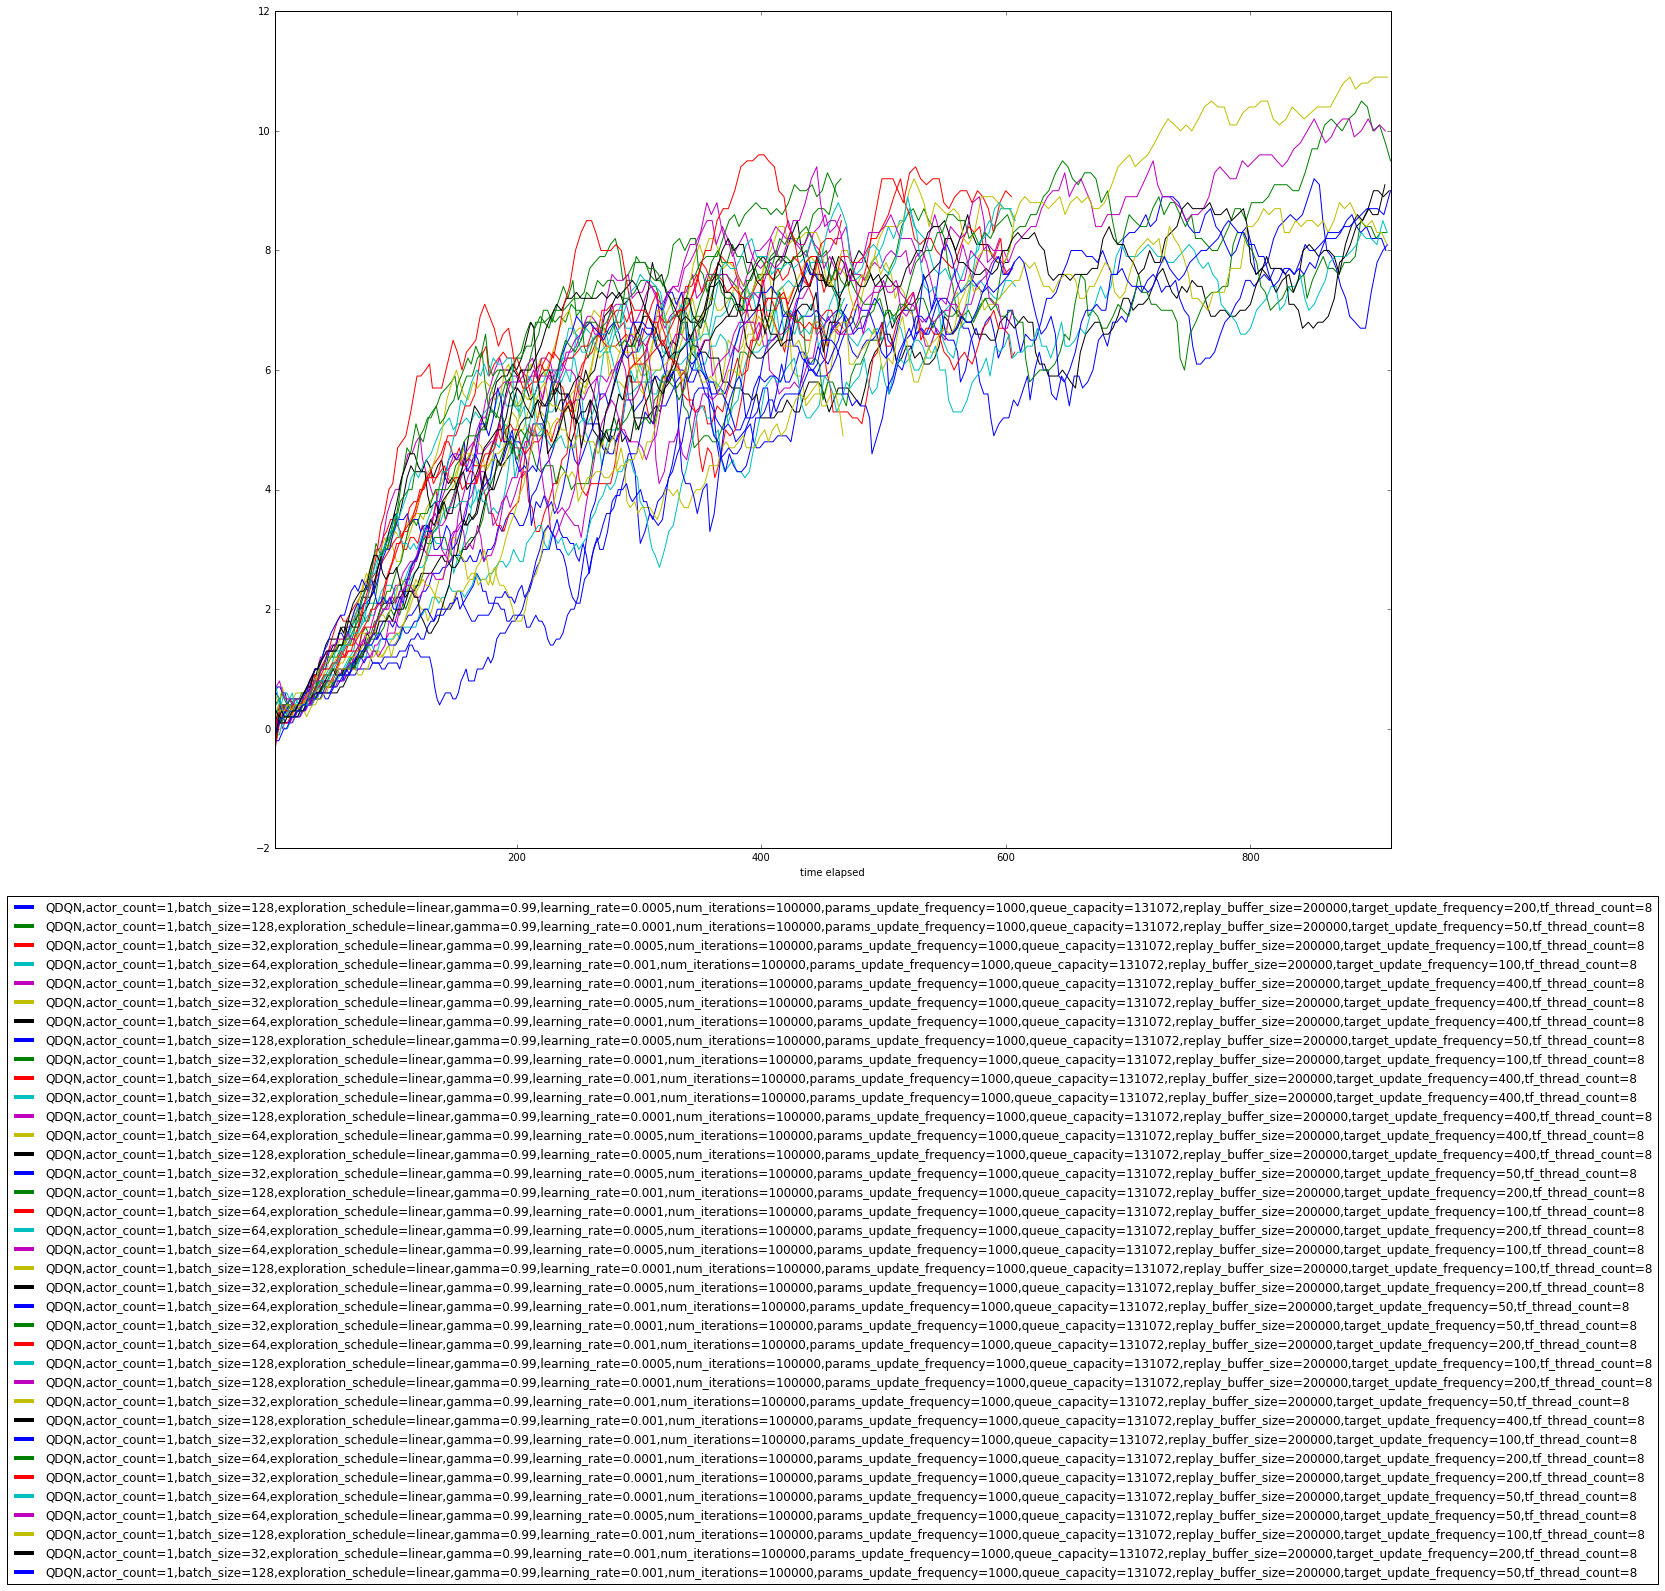
\includegraphics[height=0.35\textwidth]{doom_sweep}}
\subfloat[Quality of hyperparameters configurations]{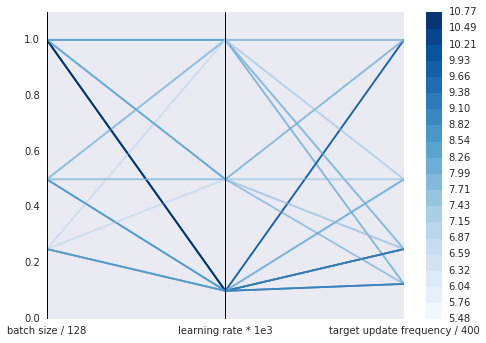
\includegraphics[height=0.35\textwidth]{sweep_parallel_coordinates}}\\
\caption{Parameter sweep for DoomDefendCenter environment}
\label{fig:doom_sweep}
\end{figure*}

\subsection{Training setup}

\begin{figure*}[t]
\subfloat[VizDoom Defend Center]{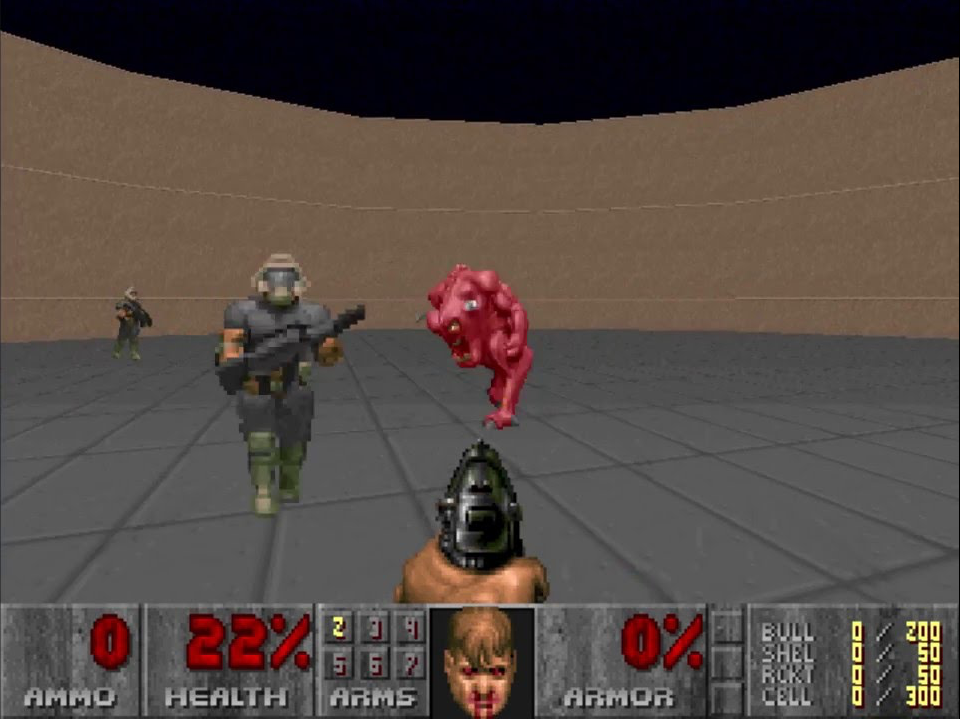
\includegraphics[height=0.35\textwidth]{vizdoom_defend_center}}\hspace{1.5cm}
\subfloat[Atari Pong]{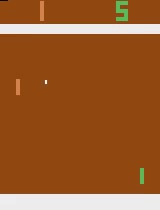
\includegraphics[height=0.35\textwidth]{atari_pong}}\\
\caption{Raw observations for the games}
\label{fig:game_frames}
\end{figure*}

\paragraph{Doom}
As a preprocessing step, we rescale images to $80 \times 80$ and transform them from RGB to greyscale.
We also introduce a frame skip of size 4, meaning that each agent action is repeated for 4 consecutive frames.
We use the replay table of size $50000$, and anneal exploration ratio $\eps$ linearly from 1 to 0.02
over the first $1/4$ of training iterations. We use learning rate of $1e-4$.

\paragraph{Atari}
We use the same input preprocessing as in \cite{mnih-dqn-2015}, involving rescaling images to $84
\times 84$ and turning them from RGB into greyscale, and also introducing a frame skip of size 4.
We use the replay table of size $200000$, and anneal exploration ratio $\eps$ linearly from 1 to 0.02
over the first $1/4$ of training iterations. We use learning rate of $1e-4$.
We show the training performance of Decoupled DQN on two Atari environments: Pong and Boxing.
The environments are provided by OpenAI Gym, with following versions: PongDeterministic-v4 and
BoxingDeterministic-v4.

\begin{figure*}[t]
\subfloat[PongDeterministic-v4]{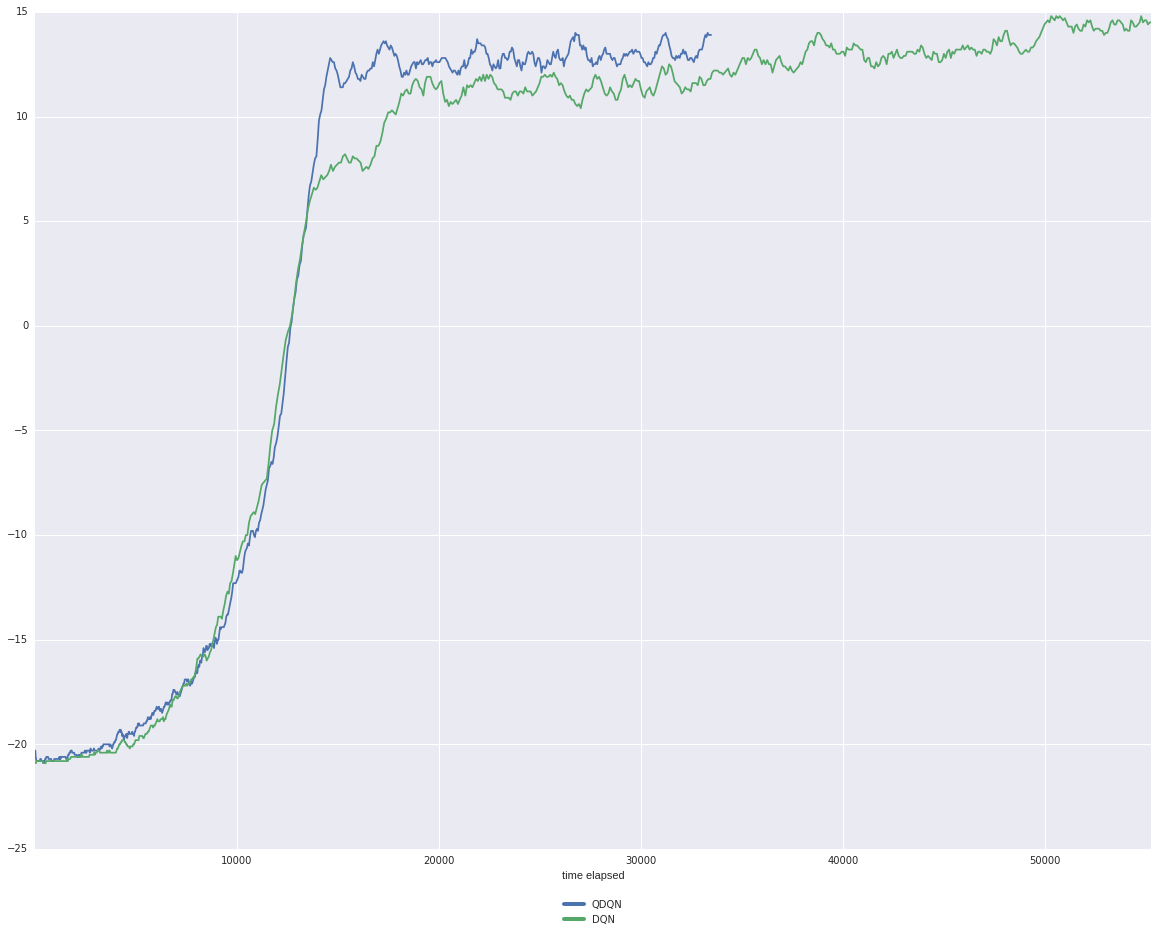
\includegraphics[width=0.5\textwidth]{pong_learning_curve}}
\subfloat[BoxingDeterministic-v4]{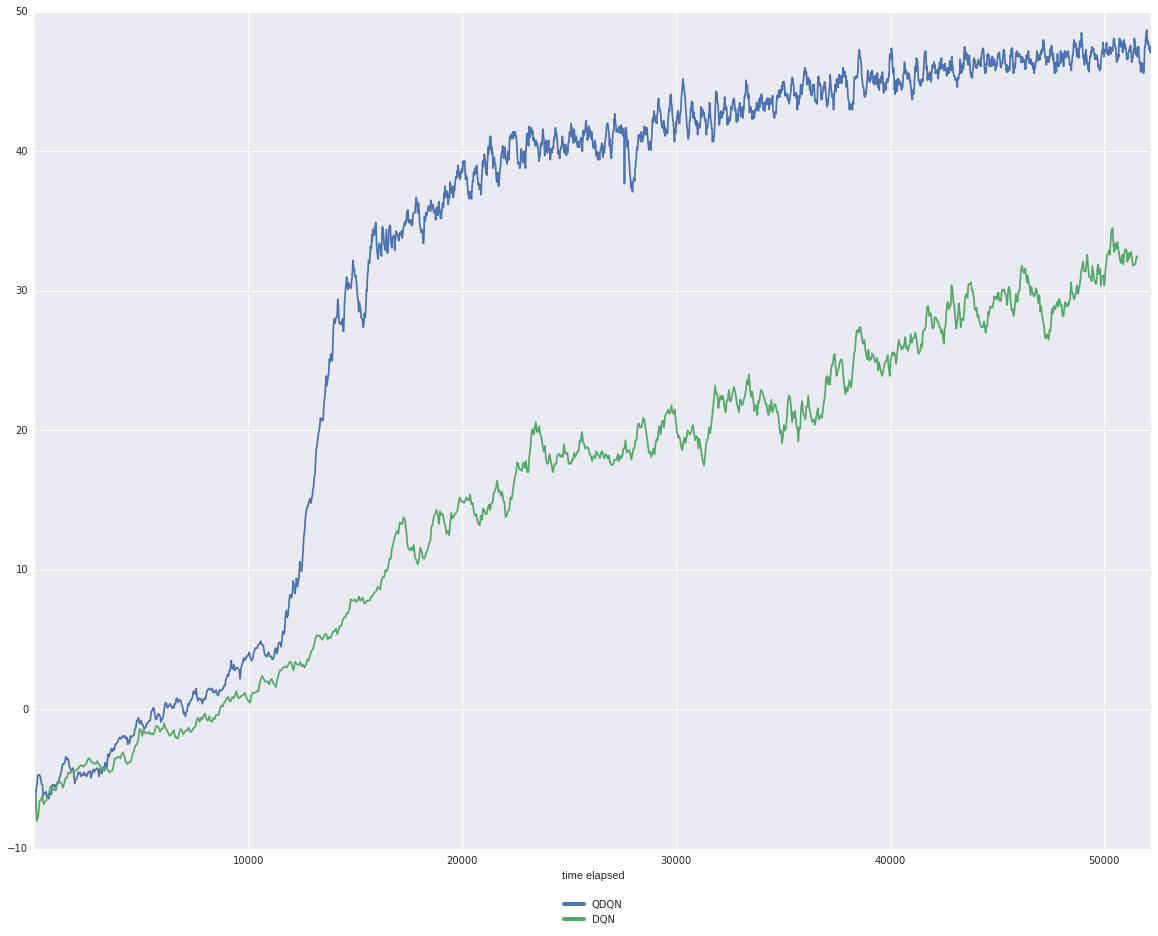
\includegraphics[width=0.5\textwidth]{boxing_learning_curve}}\\
\caption{Rewards over time for training on Atari environments (Decoupled DQN - green, DQN - blue)}
\label{fig:atari_curves}
\end{figure*}

%- Graphs of DQN, DecoupledDQN performance on 3 Atari games.

%- Explanation what is on the graph, how we made the measurements robust to the noise (choosing top 5
%from several random seeds).

%- How the methods perform in terms of wall time/sample efficiency.
